
\section{Analisi del prodotto esistente}
\hl{sezione nuovissima}

Al momento dell'arrivo in azienda è già presente una versione alpha del software. \\
Sono attualmente supportate le aziende con i codici \gls{ATECO}\G\ in ambito edilizio, permettendo di gestire le informazioni relative a:
\begin{itemize}
	\item Sedi;
	\item Cantieri;
	\item Dipendenti;
	\item Organigramma aziendale;
	\item Abitabilità;
	\item Certificato di prevenzione degli incendi;
	\item \gls{DVR}\G\ e documentazione collaterale ad esso.
\end{itemize}
Il software espone una collezione di oltre 400 domande. Sulla base delle risposte a queste domande ed alle informazioni relative alle entità sopra indicate, vengono verificate alcuni vincoli mediante delle regole del sistema esperto.


\hl{[TODO ]}

\subsection{Architettura del software}
\subsubsection{Architettura ad alto livello}
\hl{sezione nuovissima}
Il software è gestito mediante tecnologia \gls{SaaS}\G\, un modello di distribuzione del software applicativo dove il fornitore del software si occupa della sua implementazione e manutenzione. Il servizio viene erogato al cliente mediante una applicazione web fruibile via internet. \\ 
L'applicazione web risiede fisicamente su una macchina virtuale della piattaforma cloud \gls{AWS}\G\, al fine di evitare oneri e spese di gestione di una infrastruttura informatica dedicata e garantire la scalabilità del servizio.\\

Come è possibile osservare da \autoref{fig:Architettura}, ogni istanza di macchina virtuale contiene un clone dell'intera architettura. È stata scelta questa soluzione perché è prevista la possibilità di vendere il pacchetto a più utenti che possono fungere da distributori.\\
Ogni istanza è composta da tre componenti principali:
\begin{itemize}
	\item \textit{Rule Engine;}
	\item \textit{Database;}
	\item \textit{Storage.}
\end{itemize}
Il routing delle richieste viene effettuato con un \gls{reverse proxy}\G\, nello specifico \textit{NGINX}. \\
In particolare Ruby on Rails permette nativamente di creare e versionare i database a seconda dell'ambiente nel quale si opera (\textit{development, test, staging e production}). Questa caratteristica è tornata molto utile per lo sviluppo dal momento che è stato possibile fare test accurati senza intaccare i dati in produzione o utilizzare la console in sandbox di Rails la quale presenta criticità nella consistenza dei dati. \\
La persistenza dei dati è stata gestita mediante il modulo \texttt{ActiveRecord} di Ruby on Rails (descritto nella sezione \ref{sec:ActiveRecord}) salvando le informazioni su un database \textit{ PostgreSQL}.
\begin{figure}[H]
	\begin{center}
		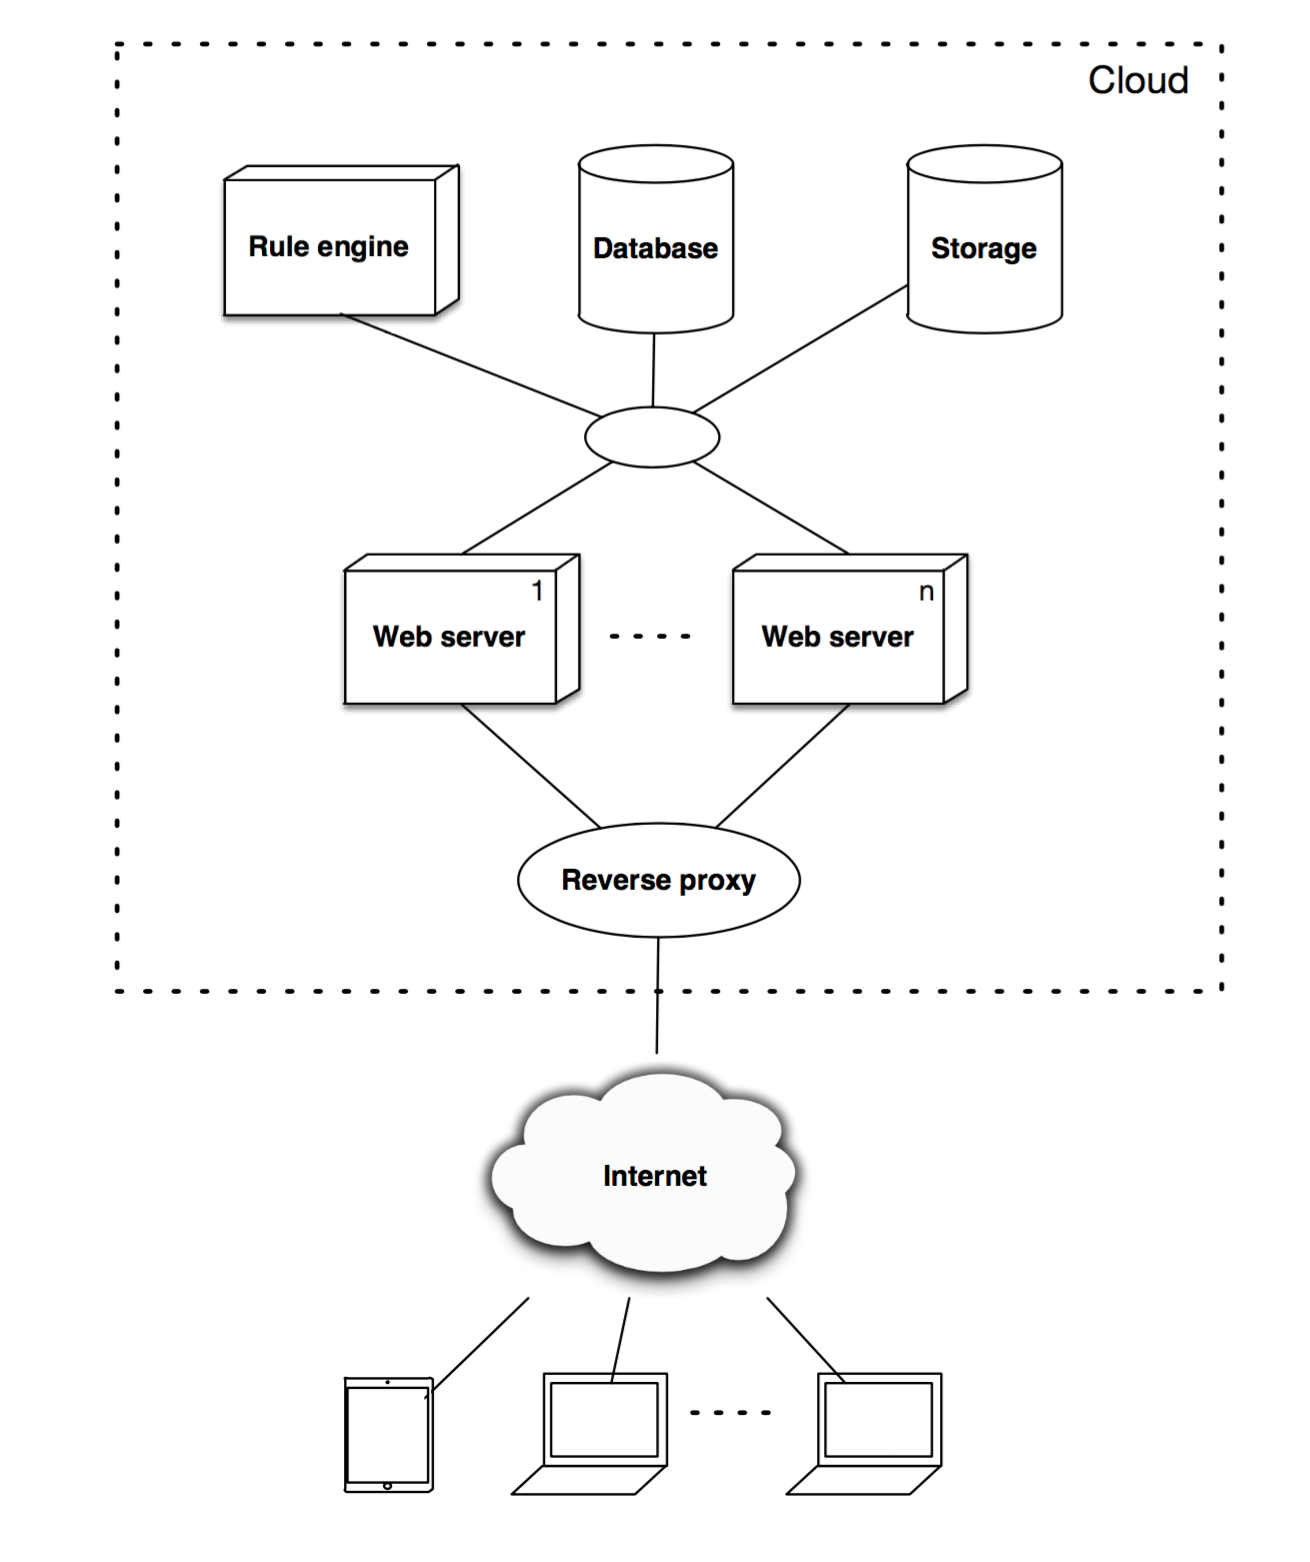
\includegraphics[width=12cm]{Pics/architettura.png}
		\caption{Architettura del sistema}
		\label{fig:Architettura}
	\end{center}
\end{figure}
\hl{SPIEGARE MEGLIO}
\subsubsection{Architettura a basso livello}
\hl{sezione nuovissima}
L'applicazione web è organizzata secondo il pattern \gls{MVC}\G\. Per il raggiungimento delle viste e l'accesso alle informazioni necessarie al corretto funzionamento dell'applicazione è stata implementata una interfaccia \gls{REST}\G\. \\
\hl{Mettere diagramma delle classi approssimativo}\\
Il sistema ha come entità principale il modello \texttt{Company} al quale sono riferite, direttamente o indirettamente, tutte le risorse.\\ 
Sono poi presenti numerosi modelli relativi alle entità che partecipano alla procedura di \gls{asseverazione}\G\.
I modelli più significativi sono:
\begin{itemize} 
	\item \texttt{Alert} per rappresentare gli allarmi;
	\item \texttt{Answer} per rappresentare le risposte alle domande;
	\item \texttt{Company} per rappresentare una azienda;
	\item \texttt{ConstructionSite} per rappresentare un cantiere;
	\item \texttt{Dpi} per rappresentare un dispositivo di protezione individuale;
	\item \texttt{Duty} per rappresentare una mansione;
	\item \texttt{FireExtinguisher}  per rappresentare un estintore;
	\item \texttt{FirstAidBox} per rappresentare una cassetta di primo soccorso;
	\item \texttt{Individual} per rappresentare una persona;
	\item \texttt{Location} per rappresentare un edificio aziendale, ovvero una sede operativa, una sede amministrativa, una sede legale oppure un magazzino;
	\item \texttt{Machine, LiftingEquipment, ElectricTool}  per rappresentare un mezzo oppure uno strumento presente nel parco macchine;
	\item \texttt{MedicalVisit} per rappresentare una visita medica;
	\item \texttt{Procedure} per rappresentare una procedura aziendale, sia essa di prassi o di sistema;
	\item \texttt{Question} per rappresentare una domanda;
	\item \texttt{Training} per rappresentare un corso.
\end{itemize}	
Per ciascun modello, sono stati realizzati opportuni \textit{controller} e \textit{viste}. \\
Sono stati implementati, inoltre numerosi \gls{concern}\G\ per modularizzare le funzionalità indipendenti dalla singola classe ed allo stesso tempo riutilizzabili da altre classi. Ad esempio, ogni modello che, se istanziato, provoca un aumento del numero delle domande in attesa di risposta, include un apposito \gls{concern}\G\ per l'aggiornamento di un contatore dedicato a tale scopo. Per l'aggiornamento del valore, il \gls{concern}\G\ ricava il nome della classe mediante \gls{reflection}\G\ sulla base dell'oggetto corrente ed incrementa il valore automaticamente del numero di domande correlate al tipo individuato.\\
\hl{[TODO finire di spiegare l'architettura ]}\\


\paragraph*{Relazioni tra domande, risposte ed allarmi}\mbox{} \\
\hl{sezione nuovissima}\\
Particolarmente degna di nota è l'associazione di una risposta o di un \textit{allarme} alla relativa risorsa. Per fare ciò si è utilizzato l'approccio di Rails per il supporto alle associazioni polimorfe, come si può vedere da  \autoref{fig:DiagrammaClassiAssociazioniPolimorfe}.\\
Nello specifico, indicando il tipo e l'id della risorsa interessata, l'accesso avviene tramite valutazione della classe e ricerca del relativo \textit{id}. \\
Si può pensare, ad esempio, all'allarme scatenato alla scadenza di un estintore. \\
La Risposta (\textit{Answer}) avrà i due campi \texttt{answerable\_type} ed \texttt{answerable\_id} impostati rispettivamente a \textit{"FireExtinguisher"} ed al suo \textit{id}.  L'allarme avrà un riferimento alla domanda per la quale è stata data una risposta. In questo modo è possibile conoscere il punto esatto dove dirottare l'utente al click sull'allarme per raggiungere il punto di non conformità. Questo aspetto è stato considerato di fondamentale importanza poiché la mole delle informazioni nel software è molto grande, è quindi necessario fornire il maggior numero di strumenti possibili all'utente per facilitarne la navigazione e l'orientamento nel sistema.
\begin{figure}[H]
	\begin{center}
		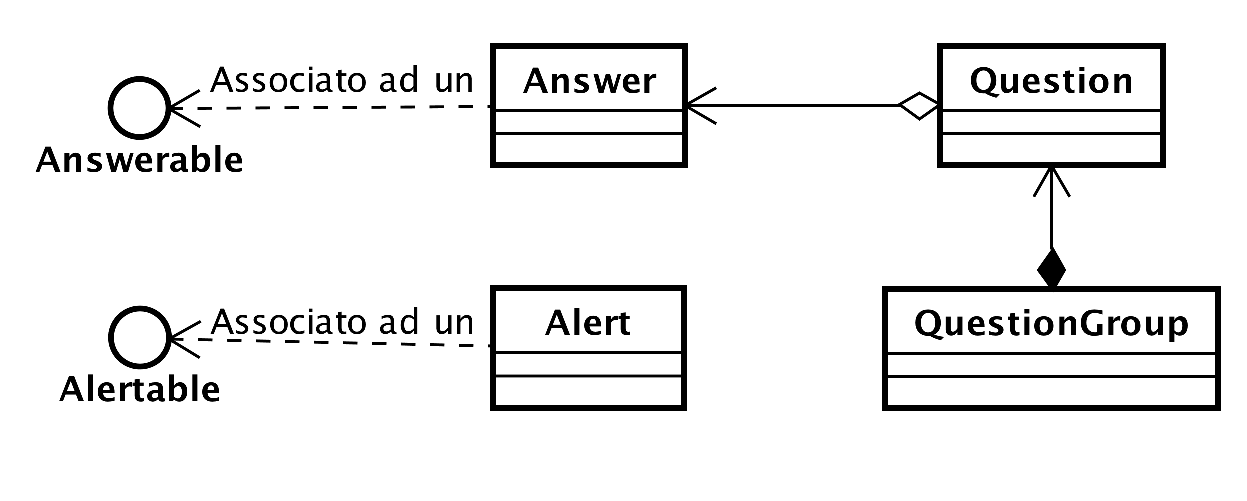
\includegraphics[width=14cm]{Pics/diagramma_classi_associazioni_polimorfe.png}
		\caption{Diagramma delle classi delle associazioni polimorfe di Risposte ed Allarmi.}
		\label{fig:DiagrammaClassiAssociazioniPolimorfe}
	\end{center}
\end{figure}

\subsubsection{Integrazione tra Ruby on Rails e Drools}\mbox{} \\
\hl{TODO scrivere meglio}
Il codice è stato scritto per la maggior parte utilizzando Ruby on Rails ma il rule engine (Drools) è un framework scritto in Java. I due linguaggi non sono nativamente compatibili. \\
Per ovviare a questo problema, è stato utilizzato JRuby, un interprete del linguaggio Ruby scritto in Java, quindi in esecuzione su una \gls{JVM}\G\. \\
Per il corretto funzionamento di Drools, è necessario inserire le informazioni nella \textit{Working Memory} come \textit{"fatti"} che sono richiesti come oggetti di tipo \gls{JavaBean}\G\ o \gls{POJO}\G\.\\
Per far cooperare i due ambienti, è stato implementato un apposito  \gls{concern}\G\ chiamato \texttt{"act\_as\_fact"}. Questo modulo viene incluso nelle classi delle quali è necessario tenere traccia nella \textit{Working Memory} e vengono generati, mediante reflection utilizzando i template di Rails (\gls{ERB}\G), le classi Java corrispondenti.




%\paragraph*{Criticità incontrate}\mbox{} \\
%\hl{SPOSTARE NELLA SEZIONE IN CUI SCRIVO QUELLO CHE HO FATTO IO}
%\hl{INSERIRE IL REMOTE TRUE NELLE VISTE}




\subsubsection{Flusso dei dati ed interazione}
\hl{Sezione nuovissima}
 Un aspetto che merita di essere esaminato è il flusso con il quale vengono generate e valutate domande e risposte  (\autoref{fig:DiagrammaAttivitaRisposte}).
\begin{figure}[H]
	\begin{center}
		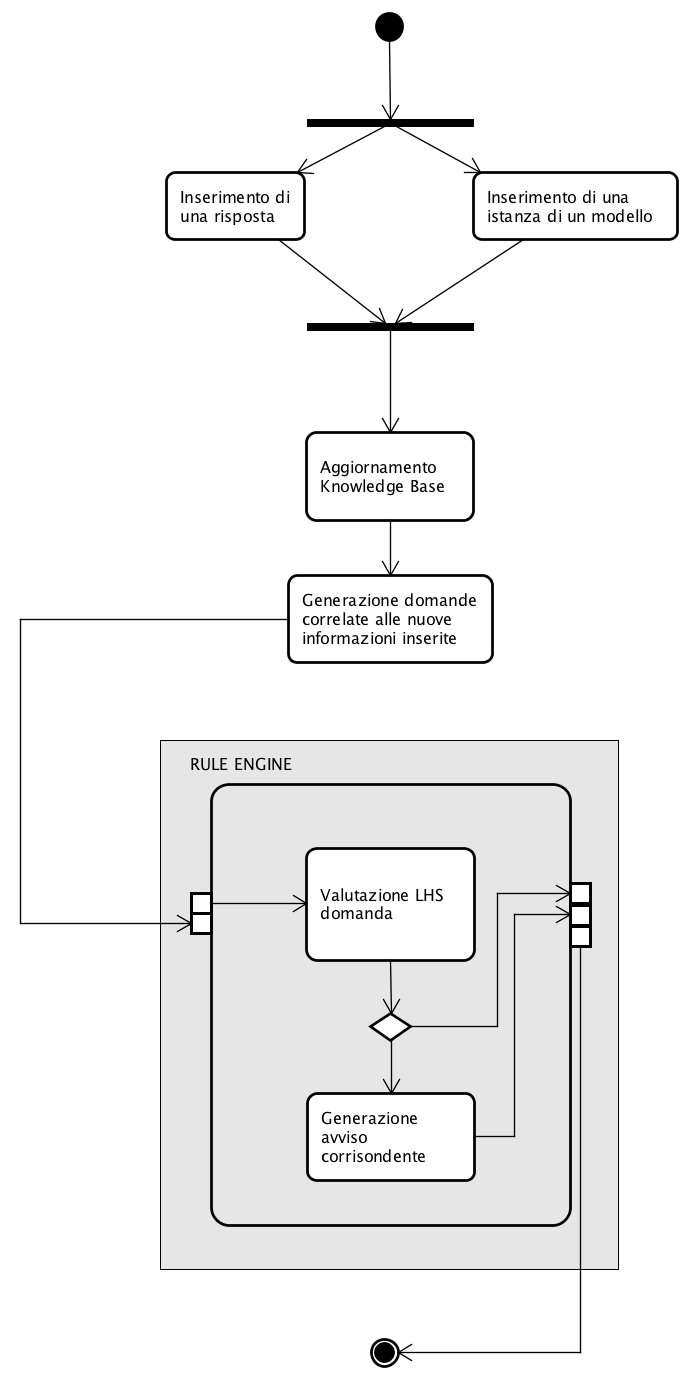
\includegraphics[width=8cm]{Pics/diagramma_attivita_risposte.png}
		\caption{Diagramma di attività del flusso di una risposta o l'inserimento di un oggetto a modello}
		\label{fig:DiagrammaAttivitaRisposte}
	\end{center}
\end{figure}

Nel momento in cui un utente inserisce o modifica un'istanza di un modello oppure risponde ad una domanda, viene aggiornata la \textit{Working Memory}. \\
Nel caso un cui venga generata o aggiornata un'istanza di modello, può essere necessario l'inserimento di alcune domande ad essa direttamente correlate.\\
Un esempio è rappresentato dall'aggiunta di un estintore ad un cantiere. Ad ogni estintore in ogni cantiere deve essere associata una posizione specifica che deve essere riportata nel layout di cantiere per permetterne il facile reperimento in caso di incendio. La posizione nel layout di un estintore è rappresentata dal software come una risposta ad una domanda in un apposito questionario generato ad ogni associazione di un estintore ad un cantiere. Se tale informazione non è specificata viene sollevato un allarme.\\
Sia per l'inserimento o aggiornamento di una risposta, sia per la generazione o modifica di una istanza di modello, il passo successivo è rappresentato dalla valutazione delle informazioni inserite sulla base della \textit{Knowledge Base}. \\
È in questo momento che agisce il rule engine Drools che per ogni regola presente nella \textit{Knowledge Base} valuta la \gls{LHS}\G\ sulle nuove informazioni inserite e, se soddisfatta, solleva gli allarmi corrispondenti. 
Un esempio di regola è il seguente:

\hl{TODO TABULAZIONI O LISTING CON AMBIENTE JAVA}
\begin{verbatim}
rule "Individuo ricopre una mansione per la quale non è formato"
	when
		$t: Training()
		$d: Duty(trainings contains $t)
		$i; Individual(duties conatins $d, trainings not contains $t)
	then
		System.out.println($i.getFirstName() + ' ' + $i.getLastName() + "ha la mansione" +
		$d.getName() + " ma non la formazione " + $t.getName() );
end
\end{verbatim}
\begin{itemize}
	\item \$t contiene tutte le formazioni;
	\item \$d contiene  tutte le mansioni che necessitano della formazione \$t;
	\item \$i contiene tutti gli individui che svolgono la mansione \$d ma non sono in possesso della formazione \$t.
\end{itemize}
Le corrispondenze di questa regola sono tutti gli individui individui che svolgono una qualunque mansione per la quale non sono correttamente formati.\\
Al verificarsi di queste condizioni, viene generato un allarme il cui contenuto è specificato dalla stampa disposta dalla \gls{RHS}\G.



\section{Definizione dei casi d'uso}
	\subsection{Legenda}
	\subsection{UC 1}
	\subsection{UC 1.1}
	\subsection{UC 1.2}
	\subsection{UC 1.2.1}
	\subsection{UC 2}	
	\subsection{UC ...}

\section{Sviluppo}
\subsection{Refactor delle componenti esistenti}
	
\subsubsection{Refactor della componente: \textit{Figure di sistema}}
\subsubsection{Refactor della componente: \textit{Dispositivi di protezione individuale}}
\subsubsection{Refactor della componente: \textit{Mansioni e formazioni correlate}}
\subsection{Refactor della componente: \textit{Questionari}}


\subsection{Nuove componenti}
\subsubsection{\textit{Segnalazioni}}
	\paragraph{Requisiti}
	\paragraph{Progettazione}
	\paragraph{Criticità incontrate}
\subsubsection{\textit{Procedure}}
	\paragraph{Requisiti}
	\paragraph{Progettazione}
	\paragraph{Criticità incontrate}
\subsubsection{\textit{Dispositivi di protezione collettivi}}
	\paragraph{Requisiti}
	\paragraph{Progettazione}
	\paragraph{Criticità incontrate}


\subsection{Regole Drools}
	
\section{Verifica e validazione}
\section{Considerazioni finali}